% vim: ts=2:sw=2:tw=80:et
\thispagestyle{fancy}
\pagestyle{fancy}

Before using specific sets of output channels (digital lines, outputs of
digital-to-analog converters, or outputs of Direct Digital Synthesis
[\acro{DDS}] devices), each output channel must be given a name, a non-waveform
static value, and have units/scaling parameters defined.  Each channel
configuration is represented by a line in the \textit{Channels} section of the
main window.  Fig.~\ref{fig:channel:select-scaling} shows two channels
configured for Arbwave use--one is a digital line used to trigger a camera and
the other is an analog voltage used to control the current in a Helmholtz coil.

\begin{figure}[ht!]
  \centerline{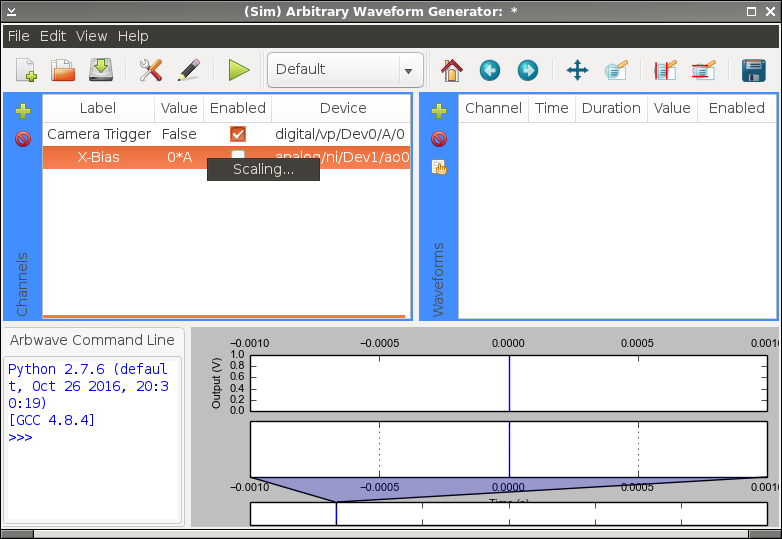
\includegraphics[width=.8\textwidth]{figures/select-scaling}}
  \caption{Having added some channels, right click an analog channel to
  specify scaling/calibration.}
  \label{fig:channel:select-scaling}
\end{figure}

\section{Channel Name}\label{sec:channels:chname}
The channel name (\textbf{Label}) is used to uniquely identify a specific output
channel using a user-specified string of characters.  The \textbf{Label} should
be used to very briefly describe the use of the particular physical output
channel.  For example, for a digital output being used to trigger a camera, an
appropriate channel name would be \textbf{Camera Trigger}.  \textbf{Label}
\textit{must} be unique with respect to all other enabled channels.

\section{Specifying Device}\label{sec:channels:dev}
The channel device selection describes the underlying hardware device and
channel on that device that will be bound as the given \textbf{Label}.
At most one channel should be bound to an underlying hardware output channel for
all enabled channels.


\section{Defining Scaling and Units}\label{sec:channels:scaling}
Arbwave allows for non-digital channels to be scaled according to an arbitrary
monotonically decreasing/increasing function.  This allows the user to calibrate
the output of a particular channel for a particular use.  For example, if a
analog voltage output channel is used to change the frequency output of a laser,
it is more convenient for the channel to be calibrated to describe the actual
frequency changes of the laser, especially if the conversion between
analog voltage and frequency is nonlinear.

As shown in Fig.~\ref{fig:channel:select-scaling},
the user can right-click a non-digital channel in the channel menu to access the
scaling dialog.  The scaling dialog, shown in Fig.~\ref{fig:channel:scaling}, gives
access to a table of scaling values that can be used to calibrate the channel.
Fig.~\ref{fig:channel:scaling}a demonstrates a linear scaling configuration for
the Helmholtz-coil current control.


\begin{figure}[hb]
  \centerline{
    a) 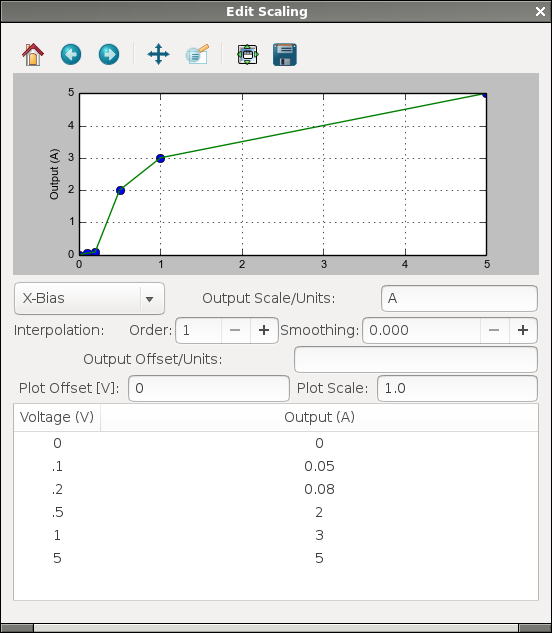
\includegraphics[width=.4\textwidth]{figures/scaling-v0}
    \hspace{.2em}
    b) 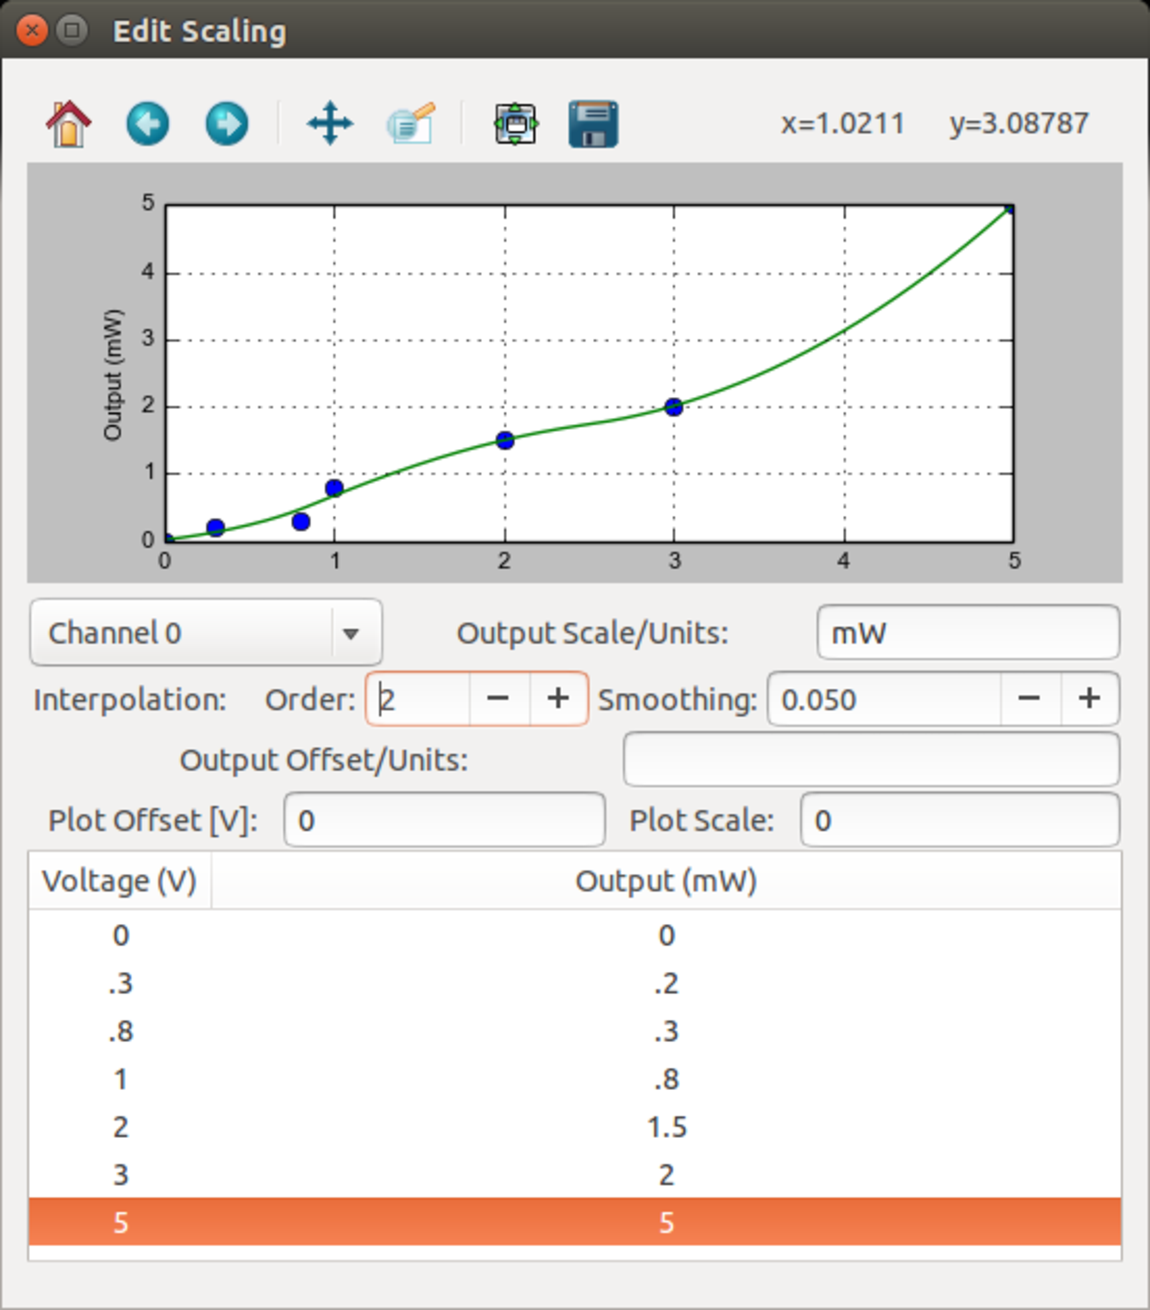
\includegraphics[width=.4\textwidth]{figures/scaling}
  }
  \caption{
    Using the scaling editor, each channel can be controlled via a set of units
    and scaling that is natural for the experiment.  a) simple linear scaling.
    b) smoothed scaling.
  }
  \label{fig:channel:scaling}
\end{figure}

As for many other inputs in Arbwave, the scaling values may be any Python
expression that evaluates to either a single value or a list of values.  Thus,
each row of this table consists of a list of voltage settings that produce the
corresponding list of output values (such as laser frequency).  The list in each
column of each row may include one or more items although it is critical that
the two cells of a row must contain the same number of elements.

In addition to simple scaling, as shown in Fig.~\ref{fig:channel:scaling}b, it is
also possible to apply a $n^{\rm th}$-order smoothing function to the data.
This may be helpful if the calibration data is somewhat noisy.

\textbf{Caution:}  it should be noted that the most predictable behavior for the
scaling table will occur when the function form of the scaling is monotonic.  If
the user enters a non-monotonic functional form, the resulting output may be
somewhat erratic.

\section{Static Values}\label{sec:channels:static}
Each configured channel must also have a \textit{static} \textbf{Value}
associated with it.  This value defines output of a channel when
the system is not operating in waveform mode (see Chap.~\ref{chap:waveforms}).
\textbf{Value} must be expressed in the proper units associated with the output
channel.  For example, a digital channel can use any expression that can be
converted to a Python boolean value.  A non-digital channel, on the other hand,
must have the dimensions as defined in the \textit{Output Scale/Units} input of
the scaling dialog.  Fig.\ref{fig:channel:select-scaling} demonstrates this
requirement by specifying \textbf{Value} as \texttt{0*A} for the
\underline{X-Bias} channel.  Be aware that output text, such as that produced in
the command line window, will typically decompose
any composite units (e.g. Pa) to a product of its base SI components (e.g.
$\mathrm{kg}*\mathrm{m}^{-1}*\mathrm{s}^{-2}$).

\section{Enabling}\label{sec:channels:enable}
Finally, each configured channel may be disabled/enabled using the
\textbf{Enabled} column checkbox.  Using this feature, it is possible to have
multiple channels defined for the same physical device output (as long as only
one is enabled at time).  This tactic is particularly helpful when determining
the scaling parameters for an analog output channel.
